
\tikzset{every picture/.style={line width=0.75pt}} %set default line width to 0.75pt        

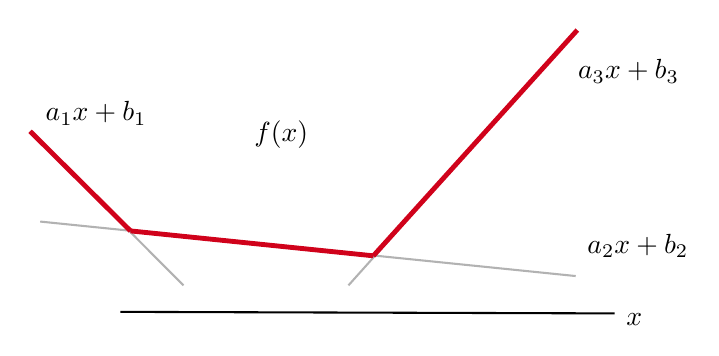
\begin{tikzpicture}[x=0.75pt,y=0.75pt,yscale=-0.75,xscale=0.75]
%uncomment if require: \path (0,300); %set diagram left start at 0, and has height of 300

%Straight Lines [id:da12023127812313228] 
\draw    (158,238) -- (475.5,239) ;
%Straight Lines [id:da35376749976820165] 
\draw  [draw opacity=0.3, line width=0.75pt]  (100,122) -- (198.5,221) ;
%Straight Lines [id:da0760682183068686] 
\draw  [draw opacity=0.3, line width=0.75pt]  (106.5,180) -- (450.5,215) ;
%Straight Lines [id:da032661760394889994] 
\draw  [draw opacity=0.3, line width=0.75pt]  (451.5,57) -- (304.5,221) ;
%Straight Lines [id:da0067101665100168795] 
\draw [color={rgb, 255:red, 208; green, 2; blue, 27 }  ,draw opacity=1, line width=1.75pt]    (320.5,202) -- (164.5,186) ;
%Straight Lines [id:da3516811366133792] 
\draw [color={rgb, 255:red, 208; green, 2; blue, 27 }  ,draw opacity=1, line width=1.75pt]    (100,122) -- (164.5,186) ;
%Straight Lines [id:da5842320764486784] 
\draw [color={rgb, 255:red, 208; green, 2; blue, 27 }  ,draw opacity=1, line width=1.75pt]    (451.5,57) -- (320.5,202) ;

% Text Node
\draw (242,113) node [anchor=north west][inner sep=0.75pt]   [align=left] {$\displaystyle f( x)$};
% Text Node
\draw (108,101) node [anchor=north west][inner sep=0.75pt]   [align=left] {$\displaystyle a_{1} x+b_{1}$};
% Text Node
\draw (456,186) node [anchor=north west][inner sep=0.75pt]   [align=left] {$\displaystyle a_{2} x+b_{2}$};
% Text Node
\draw (450,74) node [anchor=north west][inner sep=0.75pt]   [align=left] {$\displaystyle a_{3} x+b_{3}$};
% Text Node
\draw (481,237) node [anchor=north west][inner sep=0.75pt]   [align=left] {$\displaystyle x$};
\end{tikzpicture}